\documentclass[letterpaper,12pt]{article}

\usepackage{fontspec,xltxtra,xunicode}      %可使用系统自带字体
%\usepackage{}

\usepackage{setspace}    %使用行间距宏包
\usepackage{geometry}
\usepackage{graphicx}
\usepackage{amssymb}
\usepackage{indentfirst}
\usepackage{enumerate}
\usepackage{amsmath}
\usepackage{abstract}
\usepackage[slantfont, boldfont]{xeCJK}
\usepackage[colorlinks,linkcolor=black,anchorcolor=black,citecolor=black]{hyperref}
\usepackage{titlesec}
\usepackage{latexsym}
\usepackage{amsbsy}
\usepackage{amsthm}
\usepackage{amsfonts}
\usepackage{tocvsec2}
\usepackage{longtable}
\usepackage{booktabs}                % 用于表格中加下划线
\usepackage{fancyhdr}                % 页眉页脚
\usepackage{makeidx}                 % 建立索引
\usepackage{bbding}                  % 一些特殊符号
\usepackage{cite}                    % 支持引用
\usepackage{multirow}                %使用多栏宏包
\setlength{\skip\footins}{0.5cm}     % 脚注与正文的距离

\usepackage{listings}



\newcommand{\upcite}[1]{\textsuperscript{\textsuperscript{\cite{#1}}}}  %设置上标引用
\geometry{top=1.2in,bottom=1.2in,left=1.2in,right=1in}  %设置页边距
\defaultfontfeatures{Mapping=tex-text}
\XeTeXlinebreaklocale "zh"
\XeTeXlinebreakskip = 0pt plus 1pt minus 0.1pt   %设置文章内自动换行
%\setlength{\parindent}{2em}  %设定首行缩进

%中文字体设置
\setCJKmainfont[BoldFont=Adobe Heiti Std,ItalicFont=Adobe Kaiti Std]{Adobe Song Std}
\setCJKsansfont{Adobe Heiti Std}
\setCJKmonofont{Adobe Fangsong Std}
 
\setCJKfamilyfont{zhsong}{Adobe Song Std}
\setCJKfamilyfont{zhhei}{Adobe Heiti Std}
\setCJKfamilyfont{zhfs}{Adobe Fangsong Std}
\setCJKfamilyfont{zhkai}{Adobe Kaiti Std}
\setCJKfamilyfont{zhli}{LiSu}
\setCJKfamilyfont{zhyou}{YouYuan}
 
\newcommand*{\songti}{\CJKfamily{zhsong}} % 宋体
\newcommand*{\heiti}{\CJKfamily{zhhei}}   % 黑体
\newcommand*{\kaishu}{\CJKfamily{zhkai}}  % 楷书
\newcommand*{\fangsong}{\CJKfamily{zhfs}} % 仿宋
\newcommand*{\lishu}{\CJKfamily{zhli}}    % 隶书
\newcommand*{\youyuan}{\CJKfamily{zhyou}} % 幼圆

%英文字体设置
\setmainfont{Times New Roman}
\setsansfont{Arial}
\setmonofont{Consolas}

%设置字体大小
\newcommand{\chuhao}{\fontsize{42pt}{\baselineskip}\selectfont}      %初号字体
\newcommand{\xiaochu}{\fontsize{36pt}{\baselineskip}\selectfont}  %小初号字体
\newcommand{\yihao}{\fontsize{28pt}{\baselineskip}\selectfont}       %一号字体
\newcommand{\erhao}{\fontsize{21pt}{\baselineskip}\selectfont}       %二号字体
\newcommand{\xiaoer}{\fontsize{18pt}{\baselineskip}\selectfont}   %小二号字体
\newcommand{\sanhao}{\fontsize{15.75pt}{\baselineskip}\selectfont}   %三号字体
\newcommand{\sihao}{\fontsize{14pt}{\baselineskip}\selectfont}       %四号字体
\newcommand{\xiaosi}{\fontsize{12pt}{\baselineskip}\selectfont}   %小四号字体
\newcommand{\wuhao}{\fontsize{10.5pt}{\baselineskip}\selectfont}     %五号字体
\newcommand{\xiaowu}{\fontsize{9pt}{\baselineskip}\selectfont}    %小五号字体
\newcommand{\liuhao}{\fontsize{7.875pt}{\baselineskip}\selectfont}   %六号字体
\newcommand{\qihao}{\fontsize{5.25pt}{\baselineskip}\selectfont}     %七号字体

%更新目录指令
\renewcommand{\contentsname}{ \centerline {\heiti \sanhao{目\quad 录}}}
\renewcommand{\refname}{\centerline {\heiti \xiaosi{参考文献}}}


\lstset{ %  
extendedchars=false,            % Shutdown no-ASCII compatible  
language=Matlab,                % choose the language of the code  
basicstyle=\footnotesize\tt,    % the size of the fonts that are used for the code  
tabsize=3,                            % sets default tabsize to 3 spaces  
numbers=left,                   % where to put the line-numbers  
numberstyle=\tiny,              % the size of the fonts that are used for the line-numbers  
stepnumber=1,                   % the step between two line-numbers. If it's 1 each line  
                                % will be numbered  
numbersep=5pt,                  % how far the line-numbers are from the code   %  
keywordstyle=\color[rgb]{0,0,1},                % keywords  
commentstyle=\color[rgb]{0.133,0.545,0.133},    % comments  
stringstyle=\color[rgb]{0.627,0.126,0.941},      % strings  
backgroundcolor=\color{white}, % choose the background color. You must add \usepackage{color}  
showspaces=false,               % show spaces adding particular underscores  
showstringspaces=false,         % underline spaces within strings  
showtabs=false,                 % show tabs within strings adding particular underscores  
frame=single,                 % adds a frame around the code  
captionpos=b,                   % sets the caption-position to bottom  
breaklines=true,                % sets automatic line breaking  
breakatwhitespace=false,        % sets if automatic breaks should only happen at whitespace  
title=\lstname,                 % show the filename of files included with \lstinputlisting;  
                                % also try caption instead of title  
mathescape=true,escapechar=?    % escape to latex with ?..?  
escapeinside={\%*}{*)},         % if you want to add a comment within your code  
%columns=fixed,                  % nice spacing  
%morestring=[m]',                % strings  
%morekeywords={%,...},%          % if you want to add more keywords to the set  
%    break,case,catch,continue,elseif,else,end,for,function,global,%  
%    if,otherwise,persistent,return,switch,try,while,...},%  
}  




\title{Homework 5 Report}
\author{Peide Li}

\begin{document}
\maketitle

\textbf{1.} The plot of the five points is shown below:
\begin{center}
\begin{figure}[h]
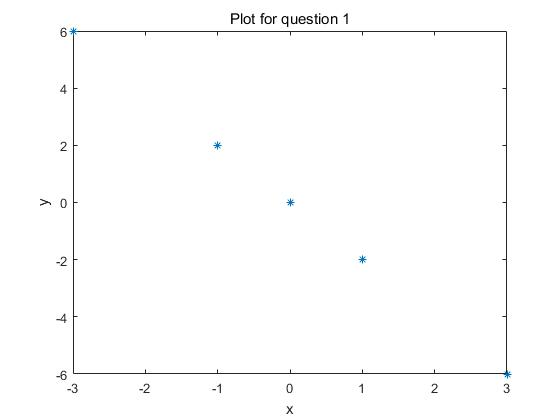
\includegraphics[width = 14cm, height = 8cm]{plot1.jpg}
\caption{Figure 1}
\end{figure}
\end{center}

The plot shows that:
\begin{itemize}
\item[1] The first principle component is $y = 0$. Because all the data are symmetrically distributed between the line $y = 0$ and the absolute value of the slop is larger than 1. So it looks more like a horizontal line than a vertical line.
\item[2] The second principle component is $x= 0$. Because all the data are also symmetrically distributed between the line $x = 0$.
\end{itemize}

\quad \\
\textbf{2.} I applied Principle component analysis to the usps data set by doing eign-decomposition to the correlation coefficient matrix of the data set. In my code, I transpose the data set A so that each column would be a data of a imagine. I use $p = 10, 50, 100, 200$ components to construct the feature spaces. And I reconstruct the first two imagines of the data set. The original first two imagines are shown here:
\begin{center}
\begin{figure}[h]
\begin{minipage}{0.48\linewidth}
  \centerline{
\includegraphics[width=4.0cm]{pca1.jpg}}
  \centerline{(a) The first imagine}
\end{minipage}
\hfill
\begin{minipage}{.48\linewidth}
  \centerline{
\includegraphics[width=4.0cm]{pca2.jpg}}
  \centerline{(b) The second imagine}
\end{minipage}
\caption{Original first two imagines}
\label{fig:res}
\end{figure}
\end{center}

And the reconstructed imagines are shown below:
\begin{center}
\begin{figure}[h]

%\begin{tabular}{cc}  
\begin{minipage}{0.48\linewidth}
  \centerline{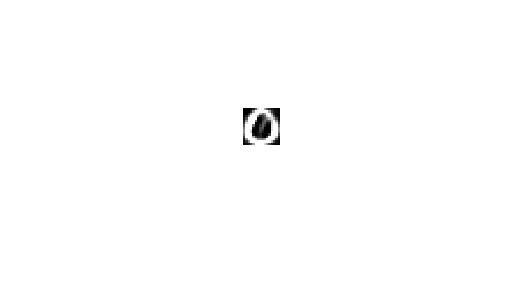
\includegraphics[width=4.0cm]{pca1_10.jpg}}
  \centerline{(a) 10 components}
\end{minipage}
\hfill
\begin{minipage}{.48\linewidth}
  \centerline{
\includegraphics[width=4.0cm]{pca1_50.jpg}}
  \centerline{(b) 50 components}
\end{minipage}
\vfill
\begin{minipage}{0.48\linewidth}
  \centerline{
\includegraphics[width=4.0cm]{pca1_100.jpg}}
  \centerline{(c) 100 components}
\end{minipage}
\hfill
\begin{minipage}{0.48\linewidth}
  \centerline{
\includegraphics[width=4.0cm]{pca1_200.jpg}}
  \centerline{(d) 200 components}
\end{minipage}
%\end{tabular}
\caption{Reconstruction of the first imagine}
\label{fig:res}

\end{figure}
\end{center}

\begin{center}
\begin{figure}[h]

%\begin{tabular}{cc}  
\begin{minipage}{0.48\linewidth}
  \centerline{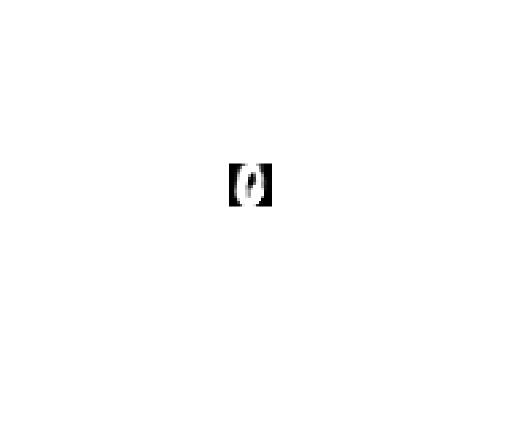
\includegraphics[width=4.0cm]{pca2_10.jpg}}
  \centerline{(a) 10 components}
\end{minipage}
\hfill
\begin{minipage}{.48\linewidth}
  \centerline{
\includegraphics[width=4.0cm]{pca2_50.jpg}}
  \centerline{(b) 50 components}
\end{minipage}
\vfill
\begin{minipage}{0.48\linewidth}
  \centerline{
\includegraphics[width=4.0cm]{pca2_100.jpg}}
  \centerline{(c) 100 components}
\end{minipage}
\hfill
\begin{minipage}{0.48\linewidth}
  \centerline{
\includegraphics[width=4.0cm]{pca2_200.jpg}}
  \centerline{(d) 200 components}
\end{minipage}
%\end{tabular}
\caption{Reconstruction of the second imagine}
\label{fig:res}

\end{figure}
\end{center}
And the total error for the reconstruction are:
\begin{center}

\begin{tabular}{c c c c c}
\hline \\
p & 10 & 50 & 100 & 200 \\
Error & $2.0920 \times 10 ^ 4$ & $1.0692\times 10 ^ 4$ & $6.2755\times 10 ^ 3$ & $1.7588\times 10 ^ 3$ \\
\hline
\end{tabular}
\end{center}
\quad \\

My code and all outcome are uploaded in my Github account:
\url{https://github.com/Kira233767/HomeWork-3.git}


\end{document}
